%==============================================================================
%  REFLEXIVE THEMATIC ANALYSIS  --  CSE 200 Lab Presentation
%  Arafat Bin A Sattar Inan (2305103) | Meherab Hossain (2305108)
%  Dipto Debnath (2305111)
%
%  COMPILE:  pdflatex rta_presentation.tex   (run twice, for the progress bar)
%            or xelatex / lualatex for the full editorial font stack
%==============================================================================
\documentclass[aspectratio=169,11pt,t]{beamer}

%------------------------------------------------------------------ 0. ENGINE
\usepackage{iftex}

%============================== CUSTOM BEAMER THEME ===========================
% (feature 16: custom colours, typography, title page, footer, spacing)

%-- 1. Editorial palette ------------------------------------------------------
\definecolor{paper}   {HTML}{F3EFE6}   % warm ivory background
\definecolor{ink}     {HTML}{202124}   % near-black primary text
\definecolor{mute}    {HTML}{6B6B67}   % muted grey secondary text
\definecolor{plum}    {HTML}{6D597A}   % muted purple
\definecolor{deepblue}{HTML}{355070}   % deep blue
\definecolor{rose}    {HTML}{B56576}   % dusty rose
\definecolor{ochre}   {HTML}{E6A65D}   % ochre
\definecolor{sage}    {HTML}{637E69}   % sage

%-- 2. Typography -------------------------------------------------------------
\ifPDFTeX
  \usepackage[T1]{fontenc}
  \usepackage[utf8]{inputenc}
  \usepackage{charter}                  % Baskerville-like serif for headings
  \usepackage[scaled=0.90]{helvet}      % humanist sans for body text
\else
  \usepackage{fontspec}
  \IfFontExistsTF{Cormorant Garamond}
    {\newfontfamily\headingfont{Cormorant Garamond}}
    {\IfFontExistsTF{Libre Baskerville}
       {\newfontfamily\headingfont{Libre Baskerville}}
       {\newfontfamily\headingfont{Latin Modern Roman}}}
  \IfFontExistsTF{Source Sans 3}
    {\setsansfont{Source Sans 3}}
    {\IfFontExistsTF{Source Sans Pro}{\setsansfont{Source Sans Pro}}{}}
  \IfFontExistsTF{IBM Plex Mono}{\setmonofont{IBM Plex Mono}}{}
\fi
\ifPDFTeX\newcommand{\headingfont}{\rmfamily}\fi

\usepackage{microtype}
\usepackage{array}
\usepackage{booktabs}                   % feature 26: professional tables
\usepackage{amsmath}                    % feature 25: conceptual notation
\usepackage{tikz}
\usetikzlibrary{positioning,calc,arrows,fit,backgrounds,%
                decorations.pathreplacing,overlay-beamer-styles}

\setbeamercolor{background canvas}{bg=paper}
\setbeamercolor{normal text}{fg=ink}
\setbeamercolor{structure}{fg=deepblue}
\setbeamercolor{frametitle}{fg=deepblue}
\setbeamercolor{itemize item}{fg=ochre}
\setbeamercolor{itemize subitem}{fg=mute}

\setbeamerfont{frametitle}{family=\headingfont,size=\LARGE,series=\mdseries}
\setbeamerfont{title}{family=\headingfont,size=\fontsize{30}{34}\selectfont}
\setbeamerfont{subtitle}{size=\normalsize}
\setbeamerfont{itemize/enumerate body}{size=\small}
\setbeamerfont{itemize/enumerate subbody}{size=\footnotesize}

\setbeamertemplate{navigation symbols}{}
\setbeamertemplate{itemize item}{\raisebox{0.12em}{\rule{0.42em}{0.42em}}}
\setbeamertemplate{itemize subitem}{\raisebox{0.18em}{\rule{0.3em}{0.9pt}}}
\setbeamertemplate{section in toc}{%
  \leavevmode\color{deepblue}\inserttocsectionnumber.~\inserttocsection\par}

%-- 3. Frame title: thin ochre rule beneath, generous whitespace --------------
\setbeamertemplate{frametitle}{%
  \vspace*{0.85em}%
  \begin{beamercolorbox}[wd=\paperwidth,leftskip=0.9cm,rightskip=0.9cm]{frametitle}
    {\usebeamerfont{frametitle}\insertframetitle}\\[0.18em]
    {\color{ochre}\rule{2.4cm}{1.1pt}}
  \end{beamercolorbox}%
  \vspace*{-0.2em}
}

%-- 4. Footer: speaker, running title, frame number + progress bar ------------
\newcommand{\currentspeaker}{}
% Total LOGICAL frames across the merged deck (Beamer counts one frame
% per \frame, not per overlay page): Part I=7 + Part II=4 + Part III=7 = 18.
% Used only to keep the footer progress bar proportional after the three
% part-PDFs are merged; each part still numbers and compiles independently.
\newcommand{\decktotalframes}{18}
\setbeamertemplate{footline}{%
  \begin{tikzpicture}[remember picture,overlay]
    \pgfmathsetmacro{\progressfrac}{\insertframenumber/\decktotalframes}
    \fill[mute!30] (0,0.66) rectangle (\paperwidth,0.735);
    \fill[ochre]   (0,0.66) rectangle (\progressfrac\paperwidth,0.735);
    \node[anchor=south west,text=mute,font=\tiny] at (0.9cm,0.16)
         {\textsc{reflexive thematic analysis}};
    \node[anchor=south,text=mute,font=\tiny] at (0.5\paperwidth,0.16)
         {\currentspeaker};
    \node[anchor=south east,text=mute,font=\tiny] at (\paperwidth-0.9cm,0.16)
         {\insertframenumber};
  \end{tikzpicture}%
  \vspace{0.95em}
}

%============================== CUSTOM COMMANDS ===============================
% (feature 17: reusable commands for recurring visual components)

\newcommand{\lede}[1]{{\color{mute}\small #1}\par\medskip}
\newcommand{\term}[1]{{\color{plum}\bfseries #1}}
\newcommand{\hl}[1]{{\color{rose}\bfseries #1}}
\newcommand{\src}[1]{\hfill{\color{mute}\scriptsize #1}}

% Big editorial pull-quote with oversized ochre quotation marks
% (feature 18: custom environment)
\newenvironment{pullquote}[1][]
  {\def\pqsource{#1}%
   \begin{center}\begin{minipage}{0.7\textwidth}
   \setlength{\leftskip}{1.1cm}%
   \noindent\hspace*{-1.1cm}%
   \raisebox{-0.42\height}[0pt][0pt]{%
     \color{ochre}\headingfont\fontsize{56}{56}\selectfont\textquotedblleft}%
   \hspace{0.18cm}%
   \color{ink}\headingfont\fontsize{17}{23}\selectfont\itshape\ignorespaces}
  {\par\vspace{0.5em}%
   \normalfont\footnotesize\color{mute}\hfill--- \pqsource
   \end{minipage}\end{center}}


% Thin-bordered "key idea" panel (feature 21: custom blocks)
\newcommand{\keyidea}[2][deepblue]{%
  \begin{tikzpicture}
    \node[draw=#1,line width=0.8pt,rounded corners=1.5pt,
          inner sep=8pt,text width=0.9\textwidth,align=center,
          font=\small,fill=#1!5] {#2};
  \end{tikzpicture}}

% Member transition slide (feature 17 + smooth hand-overs)
\newcommand{\memberslide}[5]{%
  \begin{frame}[plain]
  \begin{tikzpicture}[remember picture,overlay]
    \coordinate (O) at ([xshift=1.5cm,yshift=-2.1cm]current page.north west);
    \node[anchor=north west,text=ochre,opacity=0.32,
          font=\headingfont\fontsize{95}{95}\selectfont] at (O) {#1};
    \node[anchor=north west,text=mute,font=\scriptsize\sffamily]
          at ([xshift=3.6cm,yshift=-0.15cm]O) {PART #1};
    \node[anchor=north west,text=deepblue,text width=10.5cm,align=left,
          font=\headingfont\fontsize{25}{29}\selectfont]
          at ([xshift=3.6cm,yshift=-0.55cm]O) {#2};
    \draw[ochre,line width=1.4pt]
          ([xshift=3.65cm,yshift=-2.45cm]O) -- ([xshift=6.05cm,yshift=-2.45cm]O);
    \node[anchor=north west,text=ink,font=\normalsize\sffamily\bfseries]
          at ([xshift=3.6cm,yshift=-2.80cm]O) {#3};
    \node[anchor=north west,text=mute,font=\footnotesize\sffamily]
          at ([xshift=3.6cm,yshift=-3.40cm]O) {ID: #4};
    \node[anchor=north west,text=mute,font=\footnotesize\sffamily,
          text width=10.5cm,align=left]
          at ([xshift=3.6cm,yshift=-4.15cm]O) {#5};
  \end{tikzpicture}
  \end{frame}}

%-- Reusable TikZ styles ------------------------------------------------------
% (features 9 & 10: custom nodes + precise positioning)
\tikzset{
  card/.style={draw=mute!50,line width=0.7pt,rounded corners=2pt,
               fill=white,inner sep=7pt,text width=3.5cm,align=left,
               font=\scriptsize},
  phase/.style={circle,draw=deepblue,line width=0.9pt,fill=paper,
                minimum size=1.35cm,align=center,font=\scriptsize,text=ink},
  codebox/.style={draw=sage,line width=0.7pt,fill=sage!12,rounded corners=1.5pt,
                  inner sep=4pt,font=\scriptsize,align=left,text width=3.15cm},
  themebox/.style={draw=plum,line width=1pt,fill=plum!10,rounded corners=2pt,
                   inner sep=6pt,font=\small,align=center,text width=4.1cm},
  flow/.style={->,>=stealth,line width=0.9pt,draw=mute},
  loopback/.style={->,>=stealth,line width=0.8pt,draw=rose,dashed,
                   opacity=0.85,bend right=38},
  tag/.style={font=\tiny\sffamily,text=mute}
}

%==============================================================================
\title{Reflexive Thematic Analysis}
\subtitle{Braun \& Clarke's approach to making meaning from qualitative data}

\date{CSE 200 -- Lab Presentation}

\begin{document}
\setcounter{framenumber}{11} % continues Part I + Part II's 7+4 logical frames

%##############################################################################
\renewcommand{\currentspeaker}{Dipto Debnath \textperiodcentered\ 2305111}

\memberslide{III}{Decisions, pitfalls, quality}{Dipto Debnath}{2305111}
  {The method is flexible --- which means every choice has to be declared,
   and there are ten well-documented ways to get it wrong.}

%----------------------------------------------- Slide: the four continua ----
\begin{frame}{Four decisions you have to declare}
\vspace{-0.2em}
\lede{Reflexive TA is theoretically flexible --- but never atheoretical.
      Each choice is a position on a continuum, not a box to tick.}
\vspace{-0.9em}
\begin{center}
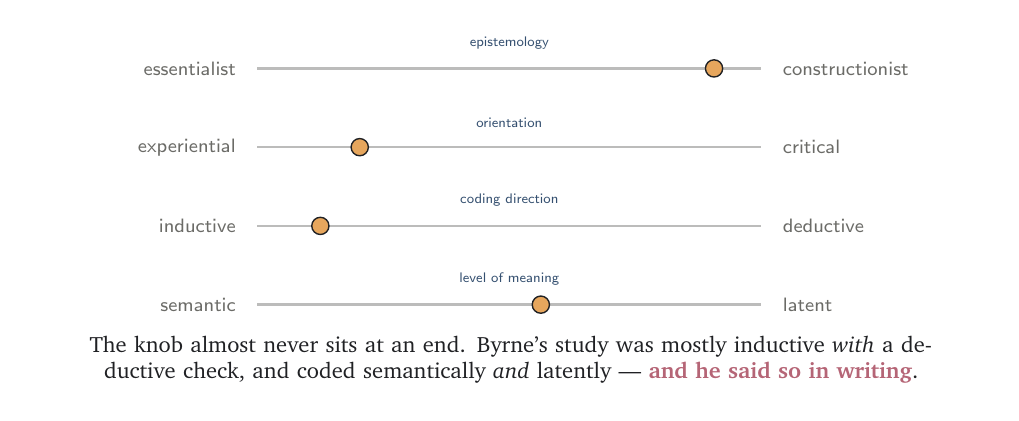
\begin{tikzpicture}[scale=1,transform shape,
  slider/.style={draw=mute!45,line width=0.9pt},
  knob/.style={circle,fill=ochre,draw=ink,line width=0.5pt,inner sep=2.2pt}]

  \foreach \y/\l/\r/\n/\pos/\ov in {
     1.7/essentialist/constructionist/epistemology/2.6/2,
     0.7/experiential/critical/orientation/-1.9/3,
    -0.3/inductive/deductive/coding direction/-2.4/4,
    -1.3/semantic/latent/level of meaning/0.4/5}
  {
    \draw[slider,visible on=<\ov->] (-3.2,\y) -- (3.2,\y);
    \node[anchor=east,font=\scriptsize\sffamily,text=mute,visible on=<\ov->]
         at (-3.35,\y) {\l};
    \node[anchor=west,font=\scriptsize\sffamily,text=mute,visible on=<\ov->]
         at (3.35,\y) {\r};
    \node[knob,visible on=<\ov->] at (\pos,\y) {};
    \node[font=\tiny\sffamily,text=deepblue,anchor=south,visible on=<\ov->]
         at (0,\y+0.12) {\n};
  }

  \node[text width=12cm,align=center,font=\footnotesize,text=ink,
        visible on=<6->] at (0,-2)
       {The knob almost never sits at an end. Byrne's study was mostly
        inductive \emph{with} a deductive check, and coded semantically
        \emph{and} latently --- \hl{and he said so in writing}.};
\end{tikzpicture}
\end{center}
\end{frame}

%-------------------------------------------- Slide: the classic mistakes ----
\begin{frame}{Ten documented problems --- three that matter most}
\vspace{-0.5em}
\begin{center}
{\scriptsize
\begin{tabular}{@{}>{\raggedright\arraybackslash}p{3.3cm}%
                 >{\raggedright\arraybackslash}p{4.3cm}%
                 >{\raggedright\arraybackslash}p{4.1cm}@{}}
\toprule
{\color{deepblue}\bfseries The problem} &
{\color{deepblue}\bfseries What it looks like} &
{\color{deepblue}\bfseries The fix} \\
\midrule
\onslide<2->{Assuming TA is one thing} &
\onslide<2->{A paper citing four incompatible TA authors at once} &
\onslide<2->{Name your variant and stick to it} \\[4pt]
\onslide<3->{Citing without reading} &
\onslide<3->{``We followed Braun \& Clarke'' --- then a codebook and a Kappa} &
\onslide<3->{Read past the 2006 paper} \\[4pt]
\onslide<4->{Topics dressed as themes} &
\onslide<4->{Themes named \emph{Benefits of\dots}, \emph{Barriers to\dots}} &
\onslide<4->{Find the shared meaning underneath} \\
\bottomrule
\end{tabular}}
\end{center}

\vspace{-1.1em}
\begin{center}
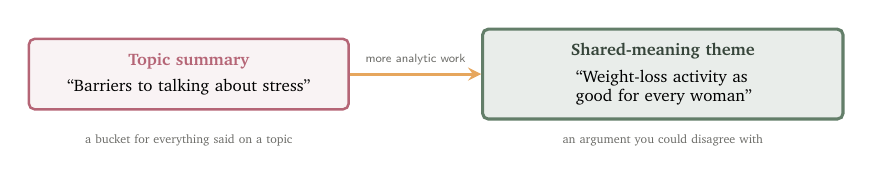
\begin{tikzpicture}[scale=0.86,transform shape]
  % before -> after (feature 14): a topic bucket becomes a real theme
  \node[draw=rose,line width=0.9pt,fill=rose!8,rounded corners=2pt,inner sep=6pt,
        text width=4.3cm,align=center,font=\scriptsize,visible on=<5->]
       (t1) at (-3.5,0) {{\color{rose}\bfseries Topic summary}\\[3pt]
        ``Barriers to talking about stress''};
  \node[draw=sage,line width=1.1pt,fill=sage!14,rounded corners=2pt,inner sep=6pt,
        text width=4.9cm,align=center,font=\scriptsize,visible on=<6->]
       (t2) at (3.5,0) {{\color{sage!55!black}\bfseries Shared-meaning theme}\\[3pt]
        ``Weight-loss activity as good for every woman''};
  \draw[->,>=stealth,line width=1.1pt,draw=ochre,visible on=<6->]
       (t1.east) -- node[above,font=\tiny\sffamily,text=mute]{more analytic work}
       (t2.west);
  \node[font=\tiny,text=mute,text width=4.3cm,align=center,visible on=<5->]
       at (-3.5,-0.98) {a bucket for everything said on a topic};
  \node[font=\tiny,text=mute,text width=4.9cm,align=center,visible on=<6->]
       at (3.5,-0.98) {an argument you could disagree with};
\end{tikzpicture}
\end{center}
\end{frame}

%--------------------------------------------------- Slide: what is quality --
\begin{frame}{So what counts as quality?}
\vspace{-0.2em}
\begin{columns}[T,onlytextwidth]
\begin{column}{0.48\textwidth}
\vspace{0.3em}
{\color{sage!55!black}\small\bfseries What quality \emph{is}}
\begin{itemize}\setlength{\itemsep}{0.1em}\small
  \item<1-> A named, justified variant of TA.
  \item<1-> Stated theoretical assumptions --- even for inductive work.
  \item<1-> Themes with a central organising concept.
  \item<1-> Extracts that are analysed, not just displayed.
\end{itemize}
\end{column}
\begin{column}{0.48\textwidth}
\vspace{0.3em}
{\color{rose}\small\bfseries What quality is \emph{not}}
\begin{itemize}\setlength{\itemsep}{0.1em}\small
  \item<2-> Inter-rater reliability scores.
  \item<2-> Consensus between coders.
  \item<2-> ``Saturation'' borrowed from grounded theory.
  \item<2-> The absence of researcher influence.
\end{itemize}
\end{column}
\end{columns}

\vspace{0.7em}
\onslide<3->{\keyidea[plum]{%
  In reflexive thematic analysis, chasing ``unbiased'' coding is not just unnecessary ---
  it is \emph{incoherent}. Subjectivity is the instrument. The published
  toolkit is a \textbf{15-point checklist} (2006) and \textbf{20 critical
  questions} for reviewers (2020).}}
\end{frame}

%------------------------------------------------------------- Slide: close --
\begin{frame}{The takeaway}
\vspace{1.2em}
\begin{pullquote}[Braun \& Clarke (2020)]
a compass and a map
\end{pullquote}
\vspace{0.4em}
\begin{center}
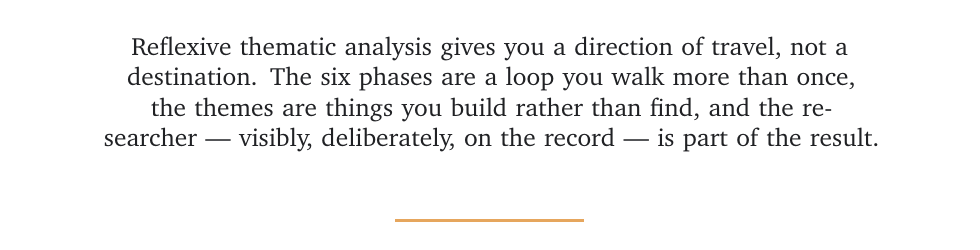
\begin{tikzpicture}
  \node[text width=11.5cm,align=center,font=\small,text=ink] {
    Reflexive thematic analysis gives you a direction of travel, not a
    destination. The six phases are a loop you walk more than once, the
    themes are things you build rather than find, and the researcher ---
    visibly, deliberately, on the record --- is part of the result.};
  \draw[ochre,line width=1pt] (-1.2,-1.6) -- (1.2,-1.6);
\end{tikzpicture}
\end{center}
\end{frame}

%--------------------------------------------------------- Slide: references --
\begin{frame}{References}
\vspace{0.4em}
{\footnotesize
\begin{thebibliography}{9}
\setbeamertemplate{bibliography item}[text]
\bibitem{bc2006} Braun, V. \& Clarke, V. (2006). Using thematic analysis in
  psychology. \emph{Qualitative Research in Psychology}, 3(2), 77--101.
\bibitem{bc2019} Braun, V. \& Clarke, V. (2019). Reflecting on reflexive
  thematic analysis. \emph{Qualitative Research in Sport, Exercise and
  Health}, 11(4), 589--597.
\bibitem{bc2020} Braun, V. \& Clarke, V. (2020). One size fits all? What
  counts as quality practice in (reflexive) thematic analysis?
  \emph{Qualitative Research in Psychology}.
\bibitem{byrne} Byrne, D. (2022). A worked example of Braun and Clarke's
  approach to reflexive thematic analysis. \emph{Quality \& Quantity},
  56, 1391--1412.
\end{thebibliography}}
\vspace{0.6em}
\begin{center}{\color{mute}\scriptsize
 Typeset in \LaTeX\ with Beamer and TikZ.}\end{center}
\end{frame}

%------------------------------------------------------------- Slide: thanks --
\begin{frame}[plain]
\begin{tikzpicture}[remember picture,overlay]
  \coordinate (K) at ([xshift=1.6cm,yshift=-3.4cm]current page.north west);
  \node[anchor=north west,text=deepblue,
        font=\headingfont\fontsize{32}{36}\selectfont] at (K) {Thank you.};
  \draw[ochre,line width=1.2pt]
       ([yshift=-1.35cm]K) -- ([xshift=2.4cm,yshift=-1.35cm]K);
  \node[anchor=north west,text=mute,font=\footnotesize\sffamily,align=left]
       at ([yshift=-1.72cm]K)
       {Arafat Bin A Sattar Inan \textperiodcentered\ 2305103 \quad
        Meherab Hossain \textperiodcentered\ 2305108 \quad
        Dipto Debnath \textperiodcentered\ 2305111};
\end{tikzpicture}
\end{frame}

\end{document}
